
\section{why executable encodings?}
\begin{frame}{executable encoding: security issues}
    \begin{itemize}
    \item malware wants to modify executables
        \begin{itemize}
        \item hide in `normal' programs (viruses)
        \item evade program analysis tools by doing weird things
        \end{itemize}
    \item memory vulnerabilities require understanding memory layout
        \begin{itemize}
        \item going from ``write memory address X'' to ``run arbitrary code''
        \item where are pointers to functions (we could change?)
        \item where is code (vulnerabilities might want to execute)
        \item where is data (vulnerabilities might want to read/change)
        \end{itemize}
    \item ways we can load+layout programs that are harder to exploit?
    \end{itemize}
\end{frame}


\section{executable and linking format (ELF)}

\usetikzlibrary{arrows.meta,calc,patterns,positioning}

\begin{frame}{memory v. disk}
\begin{tikzpicture}
\tikzset{
    mylabel/.style={font=\ttfamily},
    mybox/.style={draw,rectangle,minimum width=5cm,fill=white},
    myboxD/.style={draw,rectangle,minimum width=6cm,fill=white},
    myhigh/.style={draw,rectangle,line width=1mm, draw=blue!80!black,opacity=.3},
    nomem/.style={black!50,draw=black,fill=white},
}
\node[mybox,minimum height=1cm,pattern=north west lines,pattern color=black!20!white] (kernel) {Used by OS};
\node[above=.2cm of kernel] {(virtual) memory};
\node[mybox, minimum height=.5cm, below=1cm of kernel] (stack) {Stack};
\node[mybox, minimum height=.5cm, below=1cm of stack] (heap) {Heap / other dynamic};
\node[mybox, minimum height=.5cm, below=0mm of heap] (data) {Writable data};
\node[mybox, minimum height=.5cm, below=0mm of data] (sdata) {Code + Constants};
\coordinate (memBottom) at ($(sdata.south east) + (0mm, -2mm)$);
\begin{pgfonlayer}{bg}
\draw[pattern=north west lines, pattern color=black!40!white] (kernel.north west) rectangle (memBottom);
\end{pgfonlayer}

\node[myboxD,below right=4cm and 1cm of kernel,nomem] (diskHeader) {program header};
\node[myboxD,above=0cm of diskHeader] (textSeg) { {\tt .text} (code) };
\node[myboxD,above=0cm of textSeg] (rodataSeg) { {\tt .rodata} (read-only data) };
\node[myboxD,above=0cm of rodataSeg] (dataSeg) { {\tt .data} };
\node[myboxD,above=0cm of dataSeg,pattern=north west lines, pattern color=black!40] (bssSeg) { {\tt .bss} (zeroes; not stored) };
\node[above=.2cm of bssSeg] {program on disk};
\draw[very thick,-Latex] ([xshift=2mm]diskHeader.south east) -- ([xshift=2mm]bssSeg.north east) node[font=\small,midway,right,align=left] {higher \\ addresses \\ (and offsets)};


\foreach \f/\t in {textSeg/sdata,rodataSeg/sdata,dataSeg/data,bssSeg/data} {
    \draw[thick,-Latex,black] (\f.west) -- (\t.east);
}
\end{tikzpicture}

% FIXME: add animation: binary file format
\end{frame}

\begin{frame}{ELF (executable and linking format)}
\begin{itemize}
\item Linux {\small (and some others)} executable/object file format
\end{itemize}
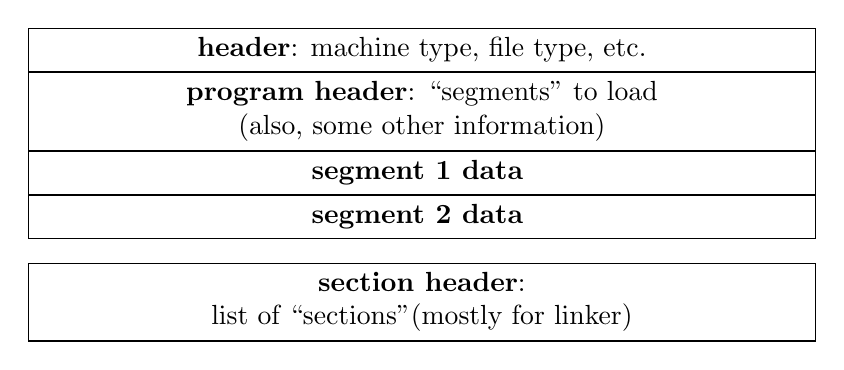
\begin{tikzpicture}
\tikzset{
    mybox/.style={draw,rectangle,minimum width=10cm,fill=white},
}
\node[mybox] (header) {
    \textbf{header}: machine type, file type, etc.
};
\node[mybox,below=0mm of header,align=center] (pHeader) {
    \textbf{program header}: ``\myemph{segments}'' to load \\
        (also, some other information)
};
\node[mybox,below=0mm of pHeader,align=center] (seg1) {
    \textbf{segment 1 data}
};
\node[mybox,below=0mm of seg1,align=center] (seg2) {
    \textbf{segment 2 data}
};
\node[mybox,below=3mm of seg2,align=center] (seg2) {
    \textbf{section header}:  \\ list of ``\myemph{sections}''(mostly for linker)
};
\end{tikzpicture}
\end{frame}

\begin{frame}{segments versus sections?}
\begin{itemize}
    \item note: ELF terminology; may not be true elsewhere!
    \item sections --- \myemph{object files} {\small (and usually executables)}, used by \myemph{linker}
        \begin{itemize}
        \item have information on intended purpose
        \item linkers combine these to create executables
        \item linkers might omit unneeded sections
        \end{itemize}
    \item segments --- executables, used to actually load program
        \begin{itemize}
        \item program loader is \myemph{dumb} --- doesn't know what segments are for
        \end{itemize}
\end{itemize}
\end{frame}



\subsection{ELF sections}

\usetikzlibrary{calc}

\begin{frame}[fragile,label=sectHeader]{section headers}
\vspace{-.25cm}
\begin{Verbatim}[fontsize=\tiny]
Sections:
Idx Name          Size      VMA               LMA               File off  Algn
  0 .note.ABI-tag 00000020  0000000000400190  0000000000400190  00000190  2**2
                  CONTENTS, ALLOC, LOAD, READONLY, DATA
  1 .note.gnu.build-id 00000024  00000000004001b0  00000000004001b0  000001b0  2**2
                  CONTENTS, ALLOC, LOAD, READONLY, DATA
  2 .rela.plt     00000210  00000000004001d8  00000000004001d8  000001d8  2**3
                  CONTENTS, ALLOC, LOAD, READONLY, DATA
  3 .init         0000001a  00000000004003e8  00000000004003e8  000003e8  2**2
                  CONTENTS, ALLOC, LOAD, READONLY, CODE
  4 .plt          00000160  0000000000400410  0000000000400410  00000410  2**4
                  CONTENTS, ALLOC, LOAD, READONLY, CODE
  5 .text         0017ff1d  0000000000400570  0000000000400570  00000570  2**4
                  CONTENTS, ALLOC, LOAD, READONLY, CODE
  6 __libc_freeres_fn 00002032  0000000000580490  0000000000580490  00180490  2**4
                  CONTENTS, ALLOC, LOAD, READONLY, CODE
  7 __libc_thread_freeres_fn 0000021b  00000000005824d0  00000000005824d0  001824d0  2**4
                  CONTENTS, ALLOC, LOAD, READONLY, CODE
  8 .fini         00000009  00000000005826ec  00000000005826ec  001826ec  2**2
                  CONTENTS, ALLOC, LOAD, READONLY, CODE
  9 .rodata       00044ac8  0000000000582700  0000000000582700  00182700  2**6
                  CONTENTS, ALLOC, LOAD, READONLY, DATA
 10 __libc_subfreeres 000000c0  00000000005c71c8  00000000005c71c8  001c71c8  2**3
                  CONTENTS, ALLOC, LOAD, READONLY, DATA
 11 .stapsdt.base 00000001  00000000005c7288  00000000005c7288  001c7288  2**0
                  CONTENTS, ALLOC, LOAD, READONLY, DATA
 12 __libc_atexit 00000008  00000000005c7290  00000000005c7290  001c7290  2**3
                  CONTENTS, ALLOC, LOAD, READONLY, DATA
 13 __libc_thread_subfreeres 00000018  00000000005c7298  00000000005c7298  001c7298  2**3
                  CONTENTS, ALLOC, LOAD, READONLY, DATA
 14 .eh_frame     000141dc  00000000005c72b0  00000000005c72b0  001c72b0  2**3
                  CONTENTS, ALLOC, LOAD, READONLY, DATA
 15 .gcc_except_table 0000020b  00000000005db48c  00000000005db48c  001db48c  2**0
                  CONTENTS, ALLOC, LOAD, READONLY, DATA
 16 .tdata        00000030  00000000007dbea8  00000000007dbea8  001dbea8  2**3
                  CONTENTS, ALLOC, LOAD, DATA, THREAD_LOCAL
 17 .tbss         0000004a  00000000007dbed8  00000000007dbed8  001dbed8  2**3
                  ALLOC, THREAD_LOCAL
 18 .init_array   00000010  00000000007dbed8  00000000007dbed8  001dbed8  2**3
                  CONTENTS, ALLOC, LOAD, DATA
 19 .fini_array   00000010  00000000007dbee8  00000000007dbee8  001dbee8  2**3
                  CONTENTS, ALLOC, LOAD, DATA
 20 .jcr          00000008  00000000007dbef8  00000000007dbef8  001dbef8  2**3
                  CONTENTS, ALLOC, LOAD, DATA
 21 .data.rel.ro  000000e8  00000000007dbf00  00000000007dbf00  001dbf00  2**6
                  CONTENTS, ALLOC, LOAD, DATA
 22 .got          00000010  00000000007dbfe8  00000000007dbfe8  001dbfe8  2**3
                  CONTENTS, ALLOC, LOAD, DATA
 23 .got.plt      000000c8  00000000007dc000  00000000007dc000  001dc000  2**3
                  CONTENTS, ALLOC, LOAD, DATA
 24 .data         00001f96  00000000007dc100  00000000007dc100  001dc100  2**6
                  CONTENTS, ALLOC, LOAD, DATA
 25 .bss          00005a90  00000000007de0c0  00000000007de0c0  001de096  2**6
                  ALLOC
 26 __libc_freeres_ptrs 00000070  00000000007e3b50  00000000007e3b50  001de096  2**3
                  ALLOC
 27 .note.stapsdt 0000100c  0000000000000000  0000000000000000  001de098  2**2
                  CONTENTS, READONLY
 28 .gnu_debuglink 00000034  0000000000000000  0000000000000000  001df0a4  2**0
                  CONTENTS, READONLY
\end{Verbatim}
\end{frame}

\begin{frame}{sections}
\begin{itemize}
\item tons of ``sections''
\item not actually needed/used to run program
\item size, file offset, flags (code/data/etc.)
    \begin{itemize}
    \item location in executable \textit{and} in memory
    \end{itemize}
\item some sections aren't stored (no ``CONTENTS'' flag) 
    \begin{itemize}
    \item just all zeroes
    \end{itemize}
\end{itemize}
\end{frame}

\begin{frame}{selected sections}
\begin{tabular}{rl}
    {\tt .text} & program code \\
    {\tt .bss} & initially zero data {\scriptsize (block started by symbol)} \\
    {\tt .data} & other writeable data  \\
    {\tt .rodata} & read-only data \\
    {\tt .init}/{\tt .fini} & global constructors/destructors \\
    {\tt .got}/{\tt .plt} & dynamic linking related \\
    {\tt .eh\_frame} & try/catch related \\
\end{tabular}
\imagecredit{based on \url{http://people.redhat.com/mpolacek/src/devconf2012.pdf}}
\end{frame}




% FIXME: something about RELOCATABLE binaries

\subsection{program headers: example static ELF binary}

\providecommand{\myemphTwo}[1]{\myemph<2>{#1}}
\providecommand{\myemphTwoB}[1]{\myemph<2>{\textbf<2>{#1}}}
\providecommand{\myemphThree}[1]{\myemph<3>{#1}}
\providecommand{\myemphFour}[1]{\myemph<4>{#1}}
\providecommand{\myemphFive}[1]{\myemph<5>{#1}}
\providecommand{\myemphSix}[1]{\myemph<6>{#1}}
\providecommand{\myemphSeven}[1]{\myemph<7>{#1}}

\begin{frame}[fragile,label=elfExOver1]{ELF example}
    \begin{itemize}
    \item {\tt objdump -x /bin/busybox} (on my laptop)
    \item {\tt -x}: output all headers
    \end{itemize}
\begin{Verbatim}[commandchars=\\\{\},fontsize=\small]
/bin/busybox:     file format \myemphTwo{elf64-x86-64}
/bin/busybox
architecture: i386:x86-64, flags 0x00000102:
EXEC_P, D_PAGED
start address \myemphThree{0x0000000000402170}

Program Header:
[...]

Sections:
[...]
\end{Verbatim}
\end{frame}

\begin{frame}[fragile,label=elfExOver2]{a program header (1)}
\begin{Verbatim}[commandchars=\\\{\},fontsize=\fontsize{9}{10}\selectfont]
Program Header:
[...]
LOAD off    0x0001000 vaddr 0x0401000 paddr 0x0401000 align 2**12
     filesz \myemphTwo{0x01b04ed} memsz 0x01b04ed flags \myemphThree{r-x}
[...]
LOAD off    0x0207950 vaddr 0x0608950 paddr 0x0608950 align 2**12
     filesz \myemphFour{0x0008f40} memsz \myemphFour{0x000c718} flags rw-

\end{Verbatim}
\begin{itemize}
\item load {\tt \myemph<2>{0x1bd04ed}} bytes:
        \begin{itemize}
        \item from {\tt 0x1000} bytes into the file 
        \item to memory at {\tt 0x401000} \\
        \item \myemph<3>{readable and executable}
        \end{itemize}
\item load {\tt 0x8f40} bytes:
        \begin{itemize}
        \item from {\tt 0x207950} bytes into the file 
        \item to memory at {\tt 0x608950} 
        \item \myemph<4>{plus ({\tt 0xc718}--{\tt 0x8f40}) bytes of zeroes}
        \item readable and writable
        \end{itemize}
\end{itemize}
\end{frame}

\begin{frame}[fragile,label=elfExOver3]{a program header (2)}
\begin{Verbatim}[commandchars=\\\{\},fontsize=\fontsize{9}{10}\selectfont]
Program Header:
[...]
    NOTE off    0x0000290 vaddr 0x0400290 paddr 0x0400290 align 2**2
         filesz 0x0000044 memsz 0x0000044 flags r--
     TLS off    0x0207950 vaddr 0x0608950 paddr 0x0608950 align 2**3
         filesz 0x0000030 memsz 0x0000092 flags r--
0x6474e553 off  0x0000270 vaddr 0x0400270 paddr 0x0400270 align 2**3
         filesz 0x0000020 memsz 0x0000020 flags r--
   STACK off    0x0000000 vaddr 0x0000000 paddr 0x0000000 align 2**4
         filesz 0x0000000 memsz 0x0000000 flags rw-
   RELRO off    0x0207950 vaddr 0x0608950 paddr 0x0608950 align 2**0
         filesz 0x00066b0 memsz 0x00066b0 flags r--
[...]
\end{Verbatim}
\begin{itemize}
\item NOTE --- comment
\item TLS --- thread-local storage region (used via {\tt \%fs})
\item 0x6474e553 --- `GNU\_PROPERTY' --- adtl linker/loader info
\item STACK --- indicates stack is read/write
\item RELRO --- make this read-only after runtime linking
\end{itemize}
\end{frame}




\subsection{ELF LOAD}
\usetikzlibrary{arrows.meta,decorations.pathmorphing,patterns}

\begin{frame}<2->{ELF LOAD}
\begin{tikzpicture}
\begin{pgfonlayer}{fg}
    \draw[very thick] (0, 0) rectangle (4, 6);
\node[font=\huge,black!25,align=center] at (2, 3) {
    program \\ on\\ disk
};
\end{pgfonlayer}
\coordinate (header tl) at (4, 0.5);
\coordinate (header br) at (0, 0);
\coordinate (load off) at (0, 1);
\coordinate (load end) at (0, 2.54);
\draw[thick,Latex-,font=\small] (0, 0) -- ++(-.5, 0) node[left,align=right] {off {\tt 0}\\ (start)};

\begin{scope}[xshift=6cm]
    \begin{pgfonlayer}{fg}
        \draw[very thick] (0, 7) -- (0, 0) -- (4, 0) -- (4, 7);
        \draw[overlay,very thick,decorate,decoration={zigzag,segment length=2.5mm}] (0, 7) -- (4, 7);
    \node[font=\huge,black!25,align=center] at (2, 3) {
        program \\ in\\ memory
    };
    \end{pgfonlayer}
    \coordinate (vaddr off) at (4, 4);
    \coordinate (vaddr end copy) at (4, 5.54);
    \coordinate (vaddr end all) at (4, 6.64);
\draw[thick,Latex-,font=\small] (4, 0) -- ++(.5, 0) node[right,align=left] {addr {\tt 0}};
\end{scope}
\begin{visibleenv}<2->
    \fill[blue!30] (header tl) rectangle (header br);
    \node[align=left,font=\small\tt,anchor=north west,draw] (load) at (1, -.25) {
        LOAD off {\color{green!50!black}0x1000} vaddr {\color{violet!70}0x4000} \ldots \\
        \hspace{1cm} filesz 0x1544 memsz 0x2644 \ldots
    };
    \draw[dotted,thick] ([yshift=-1mm]header tl -| header br) -- (load.north west);
    \draw[dotted,thick] ([xshift=3cm,yshift=-1mm]header tl -| header br) -- (load.north east);
\end{visibleenv}
\begin{visibleenv}<3->
    \draw[very thick,Latex-] (load off) -- ++(-.5cm,0) node[left,font=\small] {{\color{green!50!black}\tt 0x1000}};
    \draw[very thick,Latex-] (vaddr off) -- ++ (.5cm, 0) node[right,font=\small] {{\color{violet!70}\tt 0x4000}};
    \draw[thick,Latex-Latex] ([xshift=-.15cm]load off) -- ([xshift=-.15cm]load end)
        node[midway,font=\small,left] {\tt 0x1544};
    \draw[thick,Latex-Latex] ([xshift=.15cm]vaddr off) -- ([xshift=.15cm]vaddr end copy)
        node[midway,font=\small,right] {\tt 0x1544};
    \draw[thick,Latex-Latex] ([xshift=-4.15cm]vaddr off) -- ([xshift=-4.15cm]vaddr end all)
        node[midway,font=\small,left] {\tt 0x2644};
    \fill[red!20] (load off) rectangle ([xshift=4cm]load end);
    \fill[red!20] (vaddr off) rectangle ([xshift=-4cm]vaddr end copy);
    \fill[pattern=north west lines] (vaddr end copy) rectangle ([xshift=-4cm]vaddr end all);
\end{visibleenv}
\end{tikzpicture}
\end{frame}


\subsection{position independent executables}

\providecommand{\myemphA}[1]{\myemph<1>{#1}}
\providecommand{\myemphB}[1]{\myemph<2>{#1}}
\begin{frame}[fragile,label=dl-libs]{dynamic library headers}
\begin{Verbatim}[commandchars=\\\{\},fontsize=\fontsize{9}{10}\selectfont]
/lib/x86_64-linux-gnu/libc.so.6:     file format elf64-x86-64
/lib/x86_64-linux-gnu/libc.so.6
architecture: i386:x86-64, flags 0x00000150:
HAS_SYMS, \myemphA{DYNAMIC}, D_PAGED
start address 0x00000000000271f0

Program Header:
    PHDR off    0x0000000000000040 vaddr 0x0000000000000040 paddr 0x0000000000000040 align 2**3
         filesz 0x0000000000000310 memsz 0x0000000000000310 flags r--
  INTERP off    0x00000000001c16a0 vaddr 0x00000000001c16a0 paddr 0x00000000001c16a0 align 2**4
         filesz 0x000000000000001c memsz 0x000000000000001c flags r--
    LOAD off    0x0000000000000000 vaddr \myemphB{0x0000000000000000} paddr 0x0000000000000000 align 2**12
         filesz 0x0000000000024940 memsz 0x0000000000024940 flags r--
...
\end{Verbatim}
\begin{tikzpicture}[overlay,remember picture]
\begin{visibleenv}<1>
\node[draw,very thick,anchor=south] at ([yshift=.5cm]current page.south) {
    DYNAMIC --- instead of EXEC\_P
};
\end{visibleenv}
\begin{visibleenv}<2>
\node[draw,very thick,anchor=south,align=left] at ([yshift=.5cm]current page.south) {
    specifies loading starting at address 0 \\
    but dynamic linker will actually choose a different starting address
};
\end{visibleenv}
\end{tikzpicture}
\end{frame}

\begin{frame}[fragile,label=pie-headers]{position-independent executables}
\begin{Verbatim}[commandchars=\\\{\},fontsize=\fontsize{9}{10}\selectfont]
hello.exe:     file format elf64-x86-64
hello.exe
architecture: i386:x86-64, flags 0x00000150:
HAS_SYMS, \myemphA{DYNAMIC}, D_PAGED
start address 0x0000000000001080

Program Header:
    PHDR off    0x0000000000000040 vaddr 0x0000000000000040 paddr 0x0000000000000040 align 2**3
         filesz 0x00000000000002d8 memsz 0x00000000000002d8 flags r--
  INTERP off    0x0000000000000318 vaddr 0x0000000000000318 paddr 0x0000000000000318 align 2**0
         filesz 0x000000000000001c memsz 0x000000000000001c flags r--
    LOAD off    0x0000000000000000 vaddr \myemphB{0x0000000000000000} paddr 0x0000000000000000 align 2**12
         filesz 0x00000000000005f8 memsz 0x00000000000005f8 flags r--
\end{Verbatim}
\begin{tikzpicture}[overlay,remember picture]
\begin{visibleenv}<1>
\node[draw,very thick,anchor=south,align=left] at ([yshift=.5cm]current page.south) {
    executable with headers like dynamic library \\
    ``position-independent executable'': can be loaded at any address
};
\end{visibleenv}
\end{tikzpicture}
\end{frame}


\section{aside: other formats}


\begin{frame}{other executable formats}
    \begin{itemize}
    \item PE (Portable Executable) --- Windows
    \item Mach-O --- MacOS X
    \item broadly similar to ELF
    \item differences:  
        \begin{itemize}
        \item whether segment/section distinction exists
        \item how linking/debugging info represented
        \item how program start info represented
        \end{itemize}
    \end{itemize}
\end{frame}




\section{executable startup} % FIXME: shorten?


\begin{frame}{simple executable startup}
    \begin{itemize}
    \item copy segments into memory
    \item jump to start address
    \end{itemize}
\end{frame}

\begin{frame}{executable startup code}
    \begin{itemize}
    \item Linux: executables don't start at {\tt main}
    \item why not?
        \begin{itemize}
        \item need to initialize {\tt printf}, {\tt cout}, {\tt malloc}, etc. data structures
        \item {\tt main} needs to return somewhere
        \end{itemize}
    \item compiler links in startup code
    \end{itemize}
\end{frame}




\section{dynamic linking}

\subsection{linking primer}

\usetikzlibrary{positioning}
\begin{frame}{linking}
    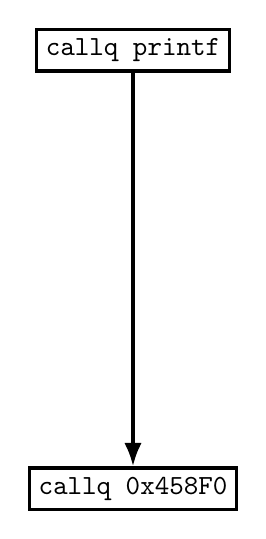
\begin{tikzpicture}
    \node[draw,font=\tt,very thick] (theCall) {callq printf};
    \node[draw,font=\tt,below=5cm of theCall,very thick] (theCallResolved) {callq 0x458F0};
    \draw[very thick,-Latex] (theCall) -- (theCallResolved);
    \end{tikzpicture}
\end{frame}

\begin{frame}{static v. dynamic linking}
    \begin{itemize}
    \item static linking --- linking \myemph{to create executable}
    \item dynamic linking --- linking \myemph{when executable is run}
    \vspace{.5cm}
    \item<2> conceptually: no difference in how they work
    \item<2> reality --- very different mechanisms
    \end{itemize}
\end{frame}

\begin{frame}{linking data structures}
    \begin{itemize}
    \item symbol table: {\tt name} $\Rightarrow$ (section, offset)
        \begin{itemize}
        \item example: {\tt main:} in assembly adds symbol table entry for {\tt main}
        \end{itemize}
    \item relocation table: offset $\Rightarrow$ (name, kind)
        \begin{itemize}
        \item example: {\tt call printf} adds relocation for name {\tt printf}
        \item kind depends on how instruction encodes address
        \end{itemize}
    \end{itemize}
\end{frame}

 % FIXME: change to have executable version

\subsubsection{in objdump, static}
\begin{frame}[fragile,label=linkingExAsm]{hello.s}
\begin{lstlisting}
.data
string: .asciz "Hello, World!"
.text
.globl main
main:
    movq $string, %rdi
    call puts
    ret
\end{lstlisting}
\end{frame}

\begin{frame}[fragile,label=linkingExObjRepeat]{hello.o (pre-static or dynamic linking)}
\begin{Verbatim}[commandchars=\\\{\},fontsize=\fontsize{9}{10}\selectfont]
SYMBOL TABLE:
0000000000000000 l    d  .text  0000000000000000 .text
0000000000000000 l    d  .data  0000000000000000 .data
0000000000000000 l    d  .bss   0000000000000000 .bss
0000000000000000 l       .data  0000000000000000 string
0000000000000000 \myemphSix{g}       \myemphSeven{.text  0000000000000000} main
0000000000000000         \myemphTwo{*UND*  0000000000000000 puts}

RELOCATION RECORDS FOR [.text]:
OFFSET           TYPE              VALUE 
0000000000000003 \myemphFive{R_X86_64_32S}      \myemphFour{.data}
0000000000000008 \myemphFive{R_X86_64_PC32}     \myemphThree{puts}-0x0000000000000004
\end{Verbatim}
\begin{tikzpicture}[overlay,remember picture]
    \tikzset{overBox/.style={at=(boxLoc),anchor=center,align=center,draw,rectangle,fill=white}}
    \coordinate (boxLoc) at ([yshift=-2.5cm]current page.center);
    \begin{visibleenv}<2>
        \node[overBox] {
            undefined symbol: look for {\tt puts} elsewhere
        };
    \end{visibleenv}
    \begin{visibleenv}<3>
        \node[overBox] {
           insert address of puts, format for {\tt call}
        };
    \end{visibleenv}
    \begin{visibleenv}<4>
        \node[overBox] {
           insert address of string, format for {\tt movq}
        };
    \end{visibleenv}
    \begin{visibleenv}<5>
        \node[overBox] {
            different ways to represent address \\
            {\tt 32S} --- signed 32-bit value \\
            {\tt PC32} --- 32-bit difference from current address
        };
    \end{visibleenv}
    \begin{visibleenv}<6>
        \node[overBox] {
            {\tt g}: global --- used by other files \\
            {\tt l}: local 
        };
    \end{visibleenv}
    \begin{visibleenv}<7>
        \node[overBox] {
            {\tt .text} segment beginning plus 0 bytes
        };
    \end{visibleenv}
\end{tikzpicture}
\end{frame}

\begin{frame}[fragile]{hello.o / statically linked, no PIE}
hello.o:
\begin{Verbatim}[commandchars=\\\{\},fontsize=\fontsize{9}{10}\selectfont]
Disassembly of section .text:

0000000000000000 <main>:
   0:   48 c7 c7 00 00 00 00    mov    $0x0,%rdi
                        3: R_X86_64_32S .data
   7:   e8 00 00 00 00          call   c <main+0xc>
                        8: R_X86_64_PLT32       puts-0x4
   c:   c3                      ret    
\end{Verbatim}
\hrule
hello.exe (gcc -static -no-pie):
\begin{Verbatim}[commandchars=\\\{\},fontsize=\fontsize{9}{10}\selectfont]
Disassembly of section .text:
...
 00000000004016c3 <main>:
   4016c3:▶      48 c7 c7 b5 16 40 00 ▶  mov    $0x4016b5,%rdi
   4016ca:▶      e8 e1 a9 00 00       ▶  call   40c0b0 <_IO_puts>
   4016cf:▶      c3                   ▶  ret    
...
\end{Verbatim}
\end{frame}



\subsection{aside: symbols in statically linked helo}
\begin{frame}[fragile]{symbols in executable}
\begin{Verbatim}[fontsize=\small]
SYMBOL TABLE:
0000000000000000 l    df *ABS*  0000000000000000 crt1.o
00000000004002b4 l     O .note.ABI-tag  0000000000000020 __abi_tag
0000000000000000 l    df *ABS*  0000000000000000 assert.o
0000000000498530 l     O .rodata        0000000000000013 errstr.0
0000000000401100 l     F .text  000000000000000f __assert_fail_base.cold
\end{Verbatim}
\ldots
\begin{itemize}
\item by default, symbol information in statically-linked executable
\item \ldots but not actually used to run it!
\vspace{.5cm}
\item can be stripped (-s linker option or strip command) isntead:
\end{itemize}
\begin{Verbatim}[fontsize=\small]
SYMBOL TABLE:
no symbols
\end{Verbatim}
\end{frame}

\begin{frame}{exercise: finding without symbols?}
\begin{itemize}
\item how can I find where functions are without symbols?
\item ideally: some \textit{automated} way to do this?
\end{itemize}
\end{frame}


\subsection{aside: strace, statically linked strace}
\begin{frame}{interlude: strace}
\begin{itemize}
\item {\tt strace} --- system call tracer
    \begin{itemize}
    \item on Linux, some other Unices
    \item OS X approx. equivalent: {\tt dtruss}
    \item Windows approx. equivalent: Process Monitor
    \end{itemize}
\item indicates what system calls (operating system services) used by a program
\end{itemize}
\end{frame}

\begin{frame}[fragile,label=staticStrace]{statically linked hello.exe}
\begin{itemize}
\item \small{\tt gcc -no-pie -static -o hello-static.exe hello.s}
\item \small{\tt strace ./hello-static.exe}:
\end{itemize}
\begin{Verbatim}[commandchars=@\{\},fontsize=\fontsize{8}{9}\selectfont]
execve("./hello-static.exe", ["./hello-static.exe"], [/* 46 vars */]) = 0
@myemphTwo{uname({sysname="Linux", nodename="reiss-lenovo", ...}) = 0}
@myemphTwo{brk(NULL)                               = 0x20a5000}
@myemphThree{brk(0x20a61c0)                          = 0x20a61c0}
@myemphTwo{arch_prctl(ARCH_SET_FS, 0x20a5880)      = 0}
@myemphTwo{readlink("/proc/self/exe", "/home/cr4bd/spring2017/cs4630/sl"..., 4096) = 62}
@myemphThree{brk(0x20c71c0)                          = 0x20c71c0}
@myemphThree{brk(0x20c8000)                          = 0x20c8000}
@myemphTwo{access("/etc/ld.so.nohwcap", F_OK)}      = -1 ENOENT (No such file or directory)
@myemphFour{fstat(1, {st_mode=S_IFCHR|0620, st_rdev=makedev(136, 1), ...}) = 0}
@myemphFour{write(1, "Hello, World!\n", 14)         = 14}
@myemphFive{exit_group(14)}                          = ?
+++ exited with 14 +++
\end{Verbatim}
\begin{tikzpicture}[overlay,remember picture]
    \tikzset{
        overBoxGeneric/.style={
            anchor=center,
            align=center,
            draw,
            rectangle,
            fill=white,
            draw=red!70!black,very thick},
        overBox/.style={
            overBoxGeneric,
            at=(boxLoc),
        },
        overBoxB/.style={
            overBoxGeneric,
            at=(boxLocB),
        },
    }
    \coordinate (boxLoc) at ([yshift=-3.5cm]current page.center);
    \begin{visibleenv}<2>
        \node[overBox] {
            standard library startup
        };
    \end{visibleenv}
    \begin{visibleenv}<3>
        \node[overBox] {
            memory allocation
        };
    \end{visibleenv}
    \begin{visibleenv}<4>
        \node[overBox] {
            implementation of puts
        };
    \end{visibleenv}
    \begin{visibleenv}<5>
        \node[overBox] {
            standard library shutdown
        };
    \end{visibleenv}
\end{tikzpicture}
\end{frame}



\subsection{example: strace hello.exe dynamic}

\begin{frame}[fragile,label=straceDynamic]{dynamically linked hello.exe}
\begin{itemize}
\item \small{\tt gcc -o hello.exe hello.s}
\item \small{\tt strace ./hello.exe}:
\end{itemize}
\begin{Verbatim}[commandchars=@\{\},fontsize=\fontsize{8}{9}\selectfont]
execve("./hello.exe", ["./hello.exe"], [/* 46 vars */]) = 0
@textit{...}
@myemphThree{mmap(NULL, 8192, PROT_READ|PROT_WRITE, MAP_PRIVATE|MAP_ANONYMOUS, -1, 0)} = 0x7fdfeeb39000
access("/etc/ld.so.preload", R_OK)      = -1 ENOENT (No such file or directory)
open("/etc/ld.so.cache", O_RDONLY|O_CLOEXEC) = 3
fstat(3, {st_mode=S_IFREG|0644, st_size=137808, ...}) = 0
@textit{...}
open("@myemphTwoB{/lib/x86_64-linux-gnu/libc.so.6}", O_RDONLY|O_CLOEXEC) = 3
@myemphFour{read(3, "\177ELF\2\1\1\3\0\0\0\0\0\0\0\0\3\0>\0\1\0\0\0P\t\2\0\0\0\0\0"..., 832) = 832}
fstat(3, {st_mode=S_IFREG|0755, st_size=1864888, ...}) = 0
@myemphFive{mmap(NULL, 3967392, PROT_READ|PROT_EXEC, ..., 3, 0) = 0x7fdfee54d000}
mprotect(0x7fdfee70c000, 2097152, PROT_NONE) = 0
@myemphFive{mmap(0x7fdfee90c000, 24576, PROT_READ|PROT_WRITE, ..., 3, 0x1bf000) = 0x7fdfee90c000}
@myemphSix{mmap(0x7fdfee912000, 14752, PROT_READ|PROT_WRITE, ..., -1, 0) = 0x7fdfee912000}
close(3)                                = 0
@textit{...}
write(1, "Hello, World!\n", 14)         = 14
exit_group(14)                          = ?
+++ exited with 14 +++
\end{Verbatim}
\begin{tikzpicture}[overlay,remember picture]
    \tikzset{overBox/.style={at=(boxLoc),anchor=center,align=center,draw,rectangle,fill=white,draw=red!70!black,very thick}}
    \coordinate (boxLoc) at ([yshift=-2cm]current page.center);
    \begin{visibleenv}<2>
        \node[overBox] {
            the standard C library (includes {\texttt{puts}})
        };
    \end{visibleenv}
    \begin{visibleenv}<3>
        \node[overBox] {
            memory allocation (different method)
        };
    \end{visibleenv}
    \begin{visibleenv}<4>
        \node[overBox] {
            read standard C library header
        };
    \end{visibleenv}
    \begin{visibleenv}<5>
        \node[overBox] {
            load standard C library ({\tt 3} = opened file)
        };
    \end{visibleenv}
    \begin{visibleenv}<6>
        \node[overBox] {
            allocate zero-initialized data segment for C library
        };
    \end{visibleenv}
\end{tikzpicture}
\end{frame}



\subsection{where's the linker}


\begin{frame}{where's the linker}
\begin{itemize}
    \item Where's the code that calls {\tt open("...libc.so.6")}?
    \item Could check {\tt hello.exe} --- it's not there!
    \vspace{.5cm}
    \item<2> instead: ``interpreter'' {\tt /lib64/ld-linux-x86-64.so.2}
    \item<2> on Linux: contains loading code instead of core OS
        \begin{itemize}
        \item OS loads it instead of program
        \end{itemize}
\end{itemize}
\end{frame}

\begin{frame}[fragile,label=interpObjdump]{objdump --- the interpreter}
\begin{itemize}
\item excerpt from {\tt objdump -sx hello.exe}:
\end{itemize}
\begin{Verbatim}[commandchars=@\{\},fontsize=\fontsize{8}{9}\selectfont]
Program Header:
@textit{...}
  INTERP off    0x0000238 vaddr 0x0@myemph{400318} paddr 0x0400238 align 2**0
         filesz 0x000001c memsz 0x000001c flags r--
@textit{...}
Contents of section .interp:
 @myemph{400318} 2f6c6962 36342f6c 642d6c69 6e75782d  @myemph{/lib64/ld-linux-}
 400328 7838362d 36342e73 6f2e3200           @myemph{x86-64.so.2}.    
\end{Verbatim}
\end{frame}


\subsection{knowing what to load?}

\begin{frame}[fragile,label=dynLinkNeeded1]{dynamic linking: what to load? (1)}
\begin{itemize}
\item excerpt from {\tt objdump -sx hello.exe}:
\end{itemize}
\begin{Verbatim}[commandchars=@\{\},fontsize=\fontsize{9}{10}\selectfont]
Program Header:
@textit{...}
 @myemph{DYNAMIC} off    0x0000000000002e20 vaddr 0x0000000000403e20 paddr 0x0000000000403e20 align 2**3
         filesz 0x00000000000001d0 memsz 0x00000000000001d0 flags rw-
@textit{...}
Dynamic Section:
  @myemph{NEEDED               libc.so.6}
  INIT                 0x0000000000401000
  ...
  STRTAB               0x0000000000400420
  ...
\end{Verbatim}
\begin{itemize}
\item program header: identifies where dynamic linking info is
\item dynamic linking info: array of key-value pairs
    \begin{itemize}
    \item needed libraries
    \item constructor locations (`INIT')
    \item string table location
    \item \ldots
    \end{itemize}
\end{itemize}
\end{frame}



\providecommand{\myemphA}[1]{\myemph<1>{#1}}
\providecommand{\myemphB}[1]{\myemph<2>{#1}}
\providecommand{\myemphAB}[1]{\myemph<1-2>{#1}}
\providecommand{\myemphC}[1]{\myemph<3>{#1}}
\begin{frame}[fragile,label=dynLinkNeeded2]{dynamic linking: what to load? (2)}
\begin{itemize}
\item excerpt from {\tt objdump -sx hello.exe}:
\end{itemize}
\begin{Verbatim}[commandchars=@\{\},fontsize=\fontsize{9}{10}\selectfont]
Program Header:
@textit{...}
 DYNAMIC off    0x0000000000002e20 vaddr @myemph{0x0000000000403e20} paddr 0x0000000000403e20 align 2**3
         filesz 0x00000000000001d0 memsz 0x00000000000001d0 flags rw-
@textit{...}
Dynamic Section:
  @myemphAB{NEEDED               libc.so.6}
  @myemphC{INIT                 0x0000000000401000}
  ...
  @myemphB{STRTAB}               0x0000000000400420
  ...
@textit{...}
 @myemphAB{403e20} @myemphA{01000000 00000000} @myemphB{01000000 00000000}  ................
 403e30 @myemphC{0c000000 00000000 00104000 00000000}  ..........@.....
\end{Verbatim}
\hrule
type \myemphA{0x1 = ``DT\_NEEDED''} (from ELF manual)\\
value \myemphB{0x1 = string table entry 1} \\
\hrule
type \myemphC{0xC = ``DT\_INIT''} \\
value \myemphC{0x401000} \\
\end{frame}

